\documentclass[12pt]{article}

\usepackage{amsmath}    % need for subequations
\usepackage{graphicx}   % need for figures
\usepackage{verbatim}   % useful for program listings
\usepackage{color}      % use if color is used in text
\usepackage{subfigure}  % use for side-by-side figures
\usepackage{hyperref}   % use for hypertext links, including those to external documents and URLs


\usepackage{graphicx}
\graphicspath{ {./images/} }

\setlength{\baselineskip}{16.0pt}    % 16 pt usual spacing between lines

\setlength{\parskip}{3pt plus 2pt}
\setlength{\parindent}{20pt}
\setlength{\oddsidemargin}{0.5cm}
\setlength{\evensidemargin}{0.5cm}
\setlength{\marginparsep}{0.75cm}
\setlength{\marginparwidth}{2.5cm}
\setlength{\marginparpush}{1.0cm}
\setlength{\textwidth}{150mm}

\begin{comment}
\pagestyle{empty} % doesn't count for page numbers
\end{comment}


\begin{document}

    \begin{titlepage}
        \begin{center}
            {\LARGE Determining the optimal orbit of polar satellites}
            \break
            {\large A Mathematical exploration}
            \break
            {\date{06.11.2018}}
            

                % ADD BREAK HERE

            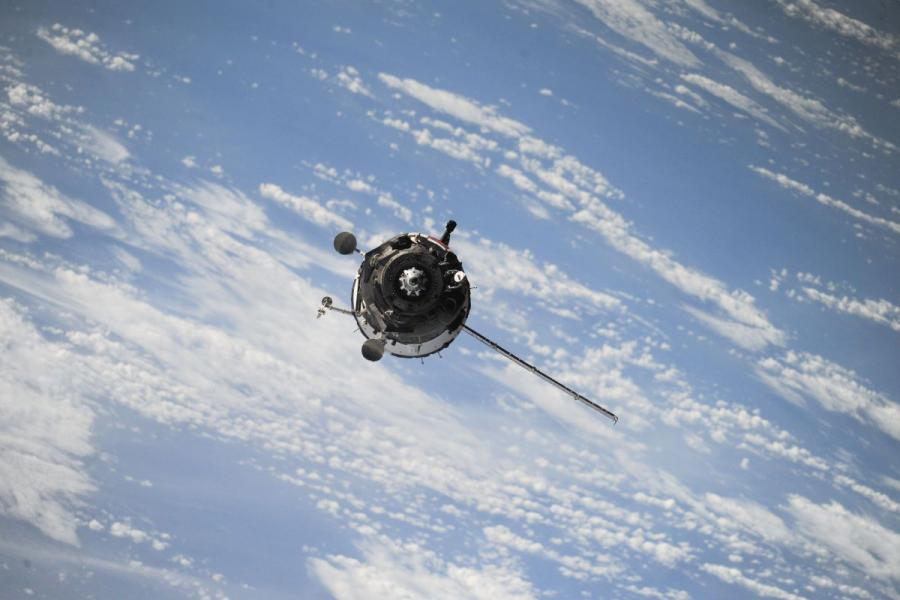
\includegraphics[scale=0.32]{pic1.jpg}
            \vspace{10pt}
            \vfill
        \end{center}
    \end{titlepage}

    \section{Introduction} % and personal engagement
    \section{Background theory}
    \section{Modelling}

    

\end{document}

